\subsection{Repetição de Experiência}

Na repetição de experiência o agente tem a possibilidade de usar uma memória de repetição que permite eficiência dos dados pela armazenação de experiências passadas do agente em ordem de ter a oportunidade de reprocessar os dados mais tarde.
Os dados salvos na memória se referem ao estado atual $s_t$, ação $a_t$, recompensa $r_t$ e próximo estado $s_{t+1}$ do agente.
Além do mais, as memórias de repetição também asseguram que as atualizações sejam feitas de dados razoavelmente estáveis guardados na memória o que na convergência da rede.

Enquanto a memória de repetição permite processar as transições de dados em diferentes ordens do que se foram experienciadas, há também a possibilidade de usar a repetição priorizada \cite{schaul2015prioritized}. Isso permite considerar transições de dados com diferentes frequências do que foram experienciadas dependendo de sua importância. Isso quer dizer, qual experiência é armazenada e qual é repetida.
A desvantagem desse método de repetição priorizada é a introdução de bias.

\subsection{Política de Gradiente}

Uma política define como um agente seleciona ações. Políticas podem ser categorizadas sobre o critério de ser tanto estacionária ou não-estacionária.
Uma política não estacionária depende no tempo de intervalo e é útil para contextos finitos onde a recompensa acumulativa que o agente procura otimizar são limitadas para um número finito de intervalos de tempo.

Políticas também podem ser categorizadas sobre um segundo critério de ser determinística ou estocástica:

\begin{itemize}
    \item No caso de ser determinística, a política é descrita por $\mu (s)$.
    \item No caso de ser estocástica, a política é descrita por $\pi (s,a)$, onde está denota a probabilidade que ação $a_t$ possa ser escolhida no estado $s_t$.
\end{itemize}

\subsubsection{Aprendizado de política-\textit{on} e política-\textit{off}}

Métodos de política-\textit{on} tentam avaliar ou melhorar a política que e usada para fazer as decisões, enquanto que o método de política-\textit{off} avalia e melhora a política diferente daquela usada para gerar dados. Em métodos baseados na política-\textit{off}, o aprendizado é bem direto quando se usa de trajetórias que necessariamente não foram obtidas sobre a política atual, mas de um diferente política de comportamento.
Nestes casos, a repetição de experiência permite o uso de experiências passadas para o aprendizado sem a introdução de bias. Ao contrário, métodos baseados na política-\textit{on} geralmente introduzem bias quando fazem uso de memórias de repetição pois as trajetórias não são obtidas somente para política atual.


% This approach is particularly well-suited
% in the case of off-policy learning as using experience from past (i.e.
% different) policies does not introduce any bias (usually it is even good
% for exploration)


\subsection{Ator-Crítica}

A política pode ser representada por redes neurais que atualizam por gradiente tanto de forma determinística ou estocástica. Para ambas formas, a política de gradiente necessita uma estimativa da função de valor da política atual. 
Uma abordagem comum é usar uma arquitetura ator-crítica, mostrada na Figura \ref{fig:actor_critic}, que consiste de duas partes: um ator e uma crítica \cite{konda2000actor}.
O ator se refere a política e a crítica para estimar a função de valor, podendo ela ser $Q(s,a)$ ou $V(s)$.
In Deep-RL, ambos o ator e a crítica podem  ser representados por aproximadores de função de rede neural não-linear.
Em resumo, pode ser dito que o a rede ator é responsável pela exploração de ações do agente no ambiente. Enquanto que para a rede da crítica é o que guia a rede ator dizendo se aquela ação é boa ou ruim. 

\begin{figure}[H]
\caption{Arquitetura Ator-Crítica}
\centerline{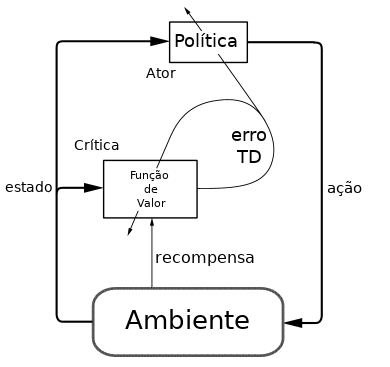
\includegraphics[width=10cm]{imagens/actor-critic_portuguese.png}}
\small{Fonte: Autor}
\label{fig:actor_critic}
\end{figure}